\section{Peer-to-Peer-Technologie}
\label{subsec:peer_to_peer_technologie}
% #TODO: Funktion des Kademlia Protokolls nennen und erklären (vielleicht in Grundlagen)
% Im Kademlia-Protokoll sind vier Funktionen definiert, die für die Suche nach
% Knoten und Werten verwendet werden. Diese Funktionen sind \texttt{FIND\_NODE},
% \texttt{FIND\_VALUE}, \texttt{PING} und \texttt{STORE}. Die Funktionen
% \texttt{FIND\_NODE} und \texttt{FIND\_VALUE} werden verwendet, um nach Knoten
% oder Werten zu suchen. Die Funktion \texttt{PING} wird verwendet, um die
% Erreichbarkeit eines Knotens zu überprüfen. Die Funktion \texttt{STORE} wird
% verwendet, um einen Wert in einem Knoten zu speichern.

Peer-to-Peer-Technologien können in zwei Kategorien unterteilt werden: Peer-to-Peer-Anwendungen und Peer-to-Peer-Infrastrukturen. Die Kategorie der Peer-to-Peer-Anwen-\\dungen umfasst den Dienst der Inhaltsverteilung, bei dem die Teilnehmer Inhalte wie Musik, Videos oder andere Dateien direkt untereinander austauschen \Parencite[730-731]{Khatibi_StructuredUnstructuredP2P}. 

Daher werden viele Peer-to-Peer schnell mit Filesharing in Verbindung bringen, da diese Technologie in der Vergangenheit vor allem dafür genutzt wurde. Das bekannteste Beispiel ist das Filesharing-Netzwerk \textit{Napster}, das 1999 von Shawn \enquote{Napster} Fanning entwickelt wurde. \textit{Napster} war das erste weit verbreitete Filesharing-Netzwerk, das auf Peer-to-Peer-Technologie basierte. Es ermöglichte den Austausch von Musikdateien zwischen den Teilnehmern. Die Musikdateien wurden dabei auf den Computern der Teilnehmer gespeichert und konnten von anderen Teilnehmern heruntergeladen werden. Da diese Art des Datenaustauschs oftmals illegal war, wurde Napster 2001 aufgrund von Urheberrechtsverletzungen abgeschaltet \parencite[S. 4-6]{Mahlmann_P2PNetzwerke}.

Die Peer-to-Peer-Infrastruktur umfasst die Peer-to-Peer-Netzwerke, die für die Kommunikation zwischen den Teilnehmern verwendet werden \parencite[S. 730-731]{Khatibi_StructuredUnstructuredP2P}. Diese Arbeit konzentriert sich auf die Peer-to-Peer-Infrastruktur, die die Kommunikation zwischen den Teilnehmern ermöglichen soll.

Im Instant-Messaging-Bereich repräsentiert das Peer-to-Peer-Modell eine dezentrale Struktur, die dabei hilft, die Kommunikation zwischen den Teilnehmern zu ermöglichen. Im Gegensatz zum Client-Server-Ansatz, bei dem ein zentraler Server die Kommunikation zwischen den Teilnehmern steuert, ermöglicht das Peer-to-Peer-Netzwerk direkte Kommunikation zwischen den Teilnehmern. Beide Modelle bringen Vor- und Nachteile mit sich. Während das Client-Server-Modell eine zentrale Instanz erfordert, um die Kommunikation zu verwalten, ist das Peer-to-Peer-Netzwerk dezentralisiert und benötigt keine solche Instanz. Die Implementierung und Wartung eines Client-Server-Modells gestalten sich einfacher im Vergleich zu einem komplexeren und aufwendigeren Peer-to-Peer-Netzwerk. Das Client-Server-Modell ist weniger flexibel, da es von einer zentralen Instanz abhängt, während das Peer-to-Peer-Netzwerk aufgrund des Fehlens dieser Instanz flexibler ist. Skalierbarkeit ist ebenfalls ein Unterschied: Das Client-Server-Modell ist durch die Kapazität des Servers begrenzt, während das Peer-to-Peer-Netzwerk auf die Kapazität der Teilnehmer zurückgreift, was seine Skalierbarkeit verbessert. In Bezug auf Sicherheit ist das Client-Server-Modell weniger robust, da es auf eine zentrale Instanz angewiesen ist, während das Peer-to-Peer-Netzwerk, das ohne solche Abhängigkeit auskommt, als sicherer gilt \parencite[S. 6-8]{Mahlmann_P2PNetzwerke}.


\subsection{Typen von Peer-to-Peer-Netzwerken}

Nicht jedes Peer-to-Peer-Netzwerk ist gleich. Es gibt verschiedene Typen von Peer-to-Peer-Netzwerken, die sich in ihrer Struktur und Funktionsweise unterscheiden. Abbildung \ref{p2p_typen} zeigt die zwei Haupttypen von Peer-to-Peer-Netzwerken: unstrukturierte und strukturierte Netzwerke \parencite[S. 362-363]{Luntovskyy_ModRechnernetze}.

\begin{center}
    \captionsetup{type=figure}
    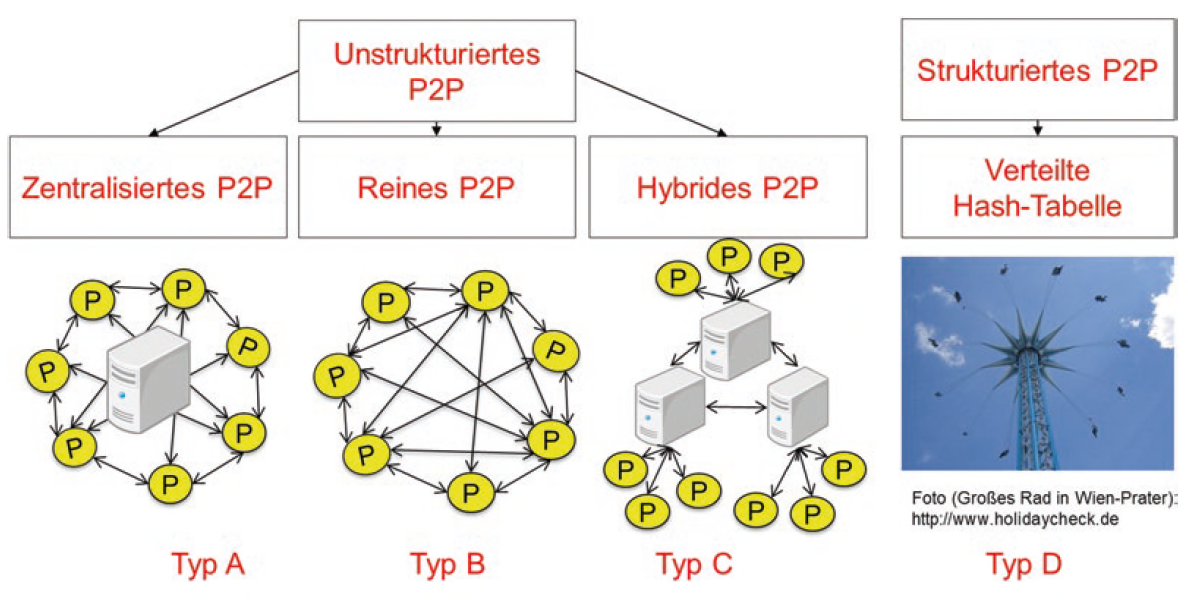
\includegraphics[width=1\linewidth]{images/peer_to_peer_typen.png}
    \captionof{figure}{Typen von Peer-to-Peer-Netzwerken \parencite{Luntovskyy_ModRechnernetze}}
    \label{p2p_typen}
\end{center}

\noindent Unstrukturierte und strukturierte Peer-to-Peer-Netzwerke sind unterschiedliche Ansätze zur Organisation von Knoten und Ressourcen in dezentralen Netzwerken.

Unstrukturierte Netzwerke sind charakterisiert durch ihre fehlende explizite Organisationsstruktur, was eine einfache Konnektivität ermöglicht. \textit{Typ A} in Abbildung \ref{p2p_typen} zeigt ein zentralisiertes Netzwerk, was bedeutet, dass alle Teilnehmer mit einem zentralen Server verbunden sind. Als Beispiel für diese Form des Peer-to-Peer dient \textit{Napster}. Bei \textit{Napster} gab es mehrere Server, die die Dateien der Teilnehmer indizierten. Die Teilnehmer konnten Dateien von anderen Teilnehmern herunterladen, indem sie eine Anfrage an einen der Server stellten, der dann die IP-Adresse des Teilnehmers zurückgab, der die Datei zur Verfügung stellte \parencite[S. 171]{Saroiu_MeasuringAndAnalyzingNapsterAndGnutellaHosts}. Diese Form ermöglicht eine schnelle und effiziente Suche nach Ressourcen, da die Ressourcen zentral verwaltet werden, aber die Abhängigkeit von einem zentralen Server macht das Netzwerk nicht skalierbar und anfällig für Ausfälle \parencite[S. 732]{Khatibi_StructuredUnstructuredP2P}.
Bei \textit{Typ B} handelt es sich um ein reines Peer-to-Peer-Netzwerk, bei dem die Teilnehmer direkt miteinander verbunden sind und jeder sowohl als Client als auch als Server fungiert \parencite[S. 732]{Khatibi_StructuredUnstructuredP2P}. Ein Beispiel für diese Form des Peer-to-Peer ist \textit{Gnutella}. Bei \textit{Gnutella} gab es keine zentrale Instanz, die die Ressourcen der Teilnehmer indizierte. Die Suche nach Ressourcen oder Informationen erfolgt durch Broadcasts oder zufällige Weiterleitungen, was jedoch zu ineffizienten Suchprozessen führen kann, da keine klare Routing-Struktur vorhanden ist \parencite[S. 171]{Saroiu_MeasuringAndAnalyzingNapsterAndGnutellaHosts}. Beim dritten und letzten Typ der unstrukturierten Netzwerke handelt es sich um ein hybrides Peer-to-Peer-Netzwerk, das Elemente aus den beiden anderen Typen kombiniert. In einem hybriden Netzwerk gibt es besondere Knoten (engl. Nodes), die die Funktionen eines Servers, wie beispielsweise Indexierung der Ressourcen, für eine bestimmte Gruppe von Teilnehmern übernehmen. Diese Knoten werden als Superknoten (engl. Super Nodes) bezeichnet. Die Super Nodes selbst sind untereinander dezentralisiert miteinander verbunden. Ein Beispiel für diese Form des Peer-to-Peer ist \textit{Gnutella2} \parencite[S. 732]{Khatibi_StructuredUnstructuredP2P}. 

Strukturierte Peer-to-Peer-Netzwerke hingegen weisen klare Regeln und Algorithmen zur Organisation der Knoten auf. Diese Netzwerke verfügen über eine explizite Organisationsstruktur, sei es eine Ringstruktur, k-bucket basierte Systeme oder andere, die es ermöglichen, effizientes Routing und eine optimierte Ressourcenverwaltung zu erreichen. Durch diese klar definierte Struktur sind strukturierte Netzwerke oft stabiler und bieten eine effizientere Ressourcenlokalisierung im Vergleich zu ihren unstrukturierten Gegenstücken. Allerdings kann diese Stabilität auf Kosten von Flexibilität und Anpassungsfähigkeit gehen, da Änderungen in der Netzwerktopologie oder hohe Dynamik der Knoten schwerer zu handhaben sind \textcolor{red}{[QUELLE]}.



\subsection{Problematik von Peer-to-Peer-Netzwerken}

Peer-to-Peer-Netzwerke sind nicht ohne Probleme. Die dezentrale Struktur der Netzwerke bringt einige Herausforderungen mit sich, die es zu bewältigen gilt. Eines der Probleme stellen die \textit{Network Address Translators} (kurz: NATs) dar. NATs sind dafür verantwortlich, dass die IP-Adressen der Teilnehmer nicht öffentlich sichtbar sind. Man unterscheidet zwischen vier verschiedenen Arten von NATs: Full Cone NAT, Restricted Cone NAT, Port Restricted Cone NAT und Symmetric NAT \parencite[S. 5]{rfc8489_STUN}. Full Cone NATs sind die einfachste Form von NATs. Sie ermöglichen es, dass ein Teilnehmer, der sich hinter einem Full Cone NAT befindet, von einem anderen Teilnehmer, der sich außerhalb des NATs befindet, erreicht werden kann, indem der Teilnehmer außerhalb des NATs eine Nachricht an den Teilnehmer hinter dem NAT sendet. Jeder Teilnehmer außerhalb des NATs kann den Teilnehmer hinter dem NAT erreichen, indem er eine Nachricht an die öffentliche IP-Adresse des NATs sendet. Das NAT leitet die Nachricht dann an den Teilnehmer hinter dem NAT weiter. Restricted Cone NATs sind ähnlich wie Full Cone NATs, mit dem Unterschied, dass nur Nachrichten von Teilnehmern akzeptiert werden, an die der Teilnehmer hinter dem NAT zuvor eine Nachricht gesendet hat. Port Restricted Cone NATs sind ähnlich wie Restricted Cone NATs, mit dem Unterschied, dass nur Nachrichten von Teilnehmern akzeptiert werden, an die der Teilnehmer hinter dem NAT zuvor eine Nachricht gesendet hat, die von demselben Port gesendet wurde, an den der Teilnehmer hinter dem NAT die Nachricht gesendet hat. Symmetric NATs sind die komplexeste Form von NATs. Sie ermöglichen es, dass ein Teilnehmer, der sich hinter einem Symmetric NAT befindet, von einem anderen Teilnehmer, der sich außerhalb des NATs befindet, erreicht werden kann, indem der Teilnehmer außerhalb des NATs eine Nachricht an den Teilnehmer hinter dem NAT sendet. Das NAT leitet die Nachricht dann an den Teilnehmer hinter dem NAT weiter. Der Teilnehmer hinter dem NAT kann jedoch nur Nachrichten von dem Teilnehmer außerhalb des NATs empfangen, an den er zuvor eine Nachricht gesendet hat.






Dies ist ein Problem, da die Teilnehmer nicht direkt miteinander kommunizieren können, wenn sie sich hinter einem NAT befinden. Um dieses Problem zu lösen, gibt es verschiedene Ansätze, wie beispielsweise STUN (Session Traversal Utilities for NAT), TURN (Traversal Using Relays around NAT) und ICE (Interactive Connectivity Establishment) \parencite[S. 1]{rfc8489_STUN}.


% #TODO: Overlay Netzwerk erklären? Kademlia ist ein Overlay Netzwerk
\begin{itemize}
    \item NAT und NAT-Problem erklären (siehe RFC 5128)
    \item Mögliche Lösungen des NAT-Problems (siehe RFC 5128)
    \item Was gibt es so für Protokolle/Algorithmen Chord, Kademlia, Pastry, Tapestry, CAN + DHTs + Churnrate
    \item ICE STUN TURN erklären
    \item Kademlia vs. Angriffe
    \item Angriffe gegen ICE gucken und erklären
\end{itemize}